% =====================================================================
%  preamble.tex -- packages, theme, colours, macros
%  Gradient Methods (CSE 402), Nawriz Ahmed Turjo, Roll 2105032
%  Engine: pdfLaTeX, no shell-escape required.
%
%  Visual system (built on Metropolis):
%    * light "paper" content slides, dark navy only for the title slide and
%      big-statement slides;
%    * three colours with fixed jobs: navy = structure, orange = attention,
%      teal = answers and key results;
%    * white frame header with a section label and an orange progress rule;
%    * numbered section dividers with a "you are here" stop strip;
%    * left-accent boxes; Part B frames carry a navy strip with the problem id.
% =====================================================================

% ---------- theme ----------
\usetheme[progressbar=none, numbering=fraction, block=fill]{metropolis}
\setbeamertemplate{frame footer}{Gradient Methods \quad|\quad Nawriz Ahmed Turjo \quad|\quad 2105032}
\setbeamersize{text margin left=0.9cm, text margin right=0.9cm}

% ---------- encoding / fonts ----------
\usepackage[T1]{fontenc}
\usepackage[utf8]{inputenc}
\usepackage[sfdefault, lining, scaled=0.92]{FiraSans}   % text
\usepackage[scaled=0.86]{FiraMono}                       % code
\renewcommand*\familydefault{\sfdefault}

% ---------- mathematics ----------
\usepackage{amsmath, amsthm, mathtools}
\usefonttheme{professionalfonts}                         % let the packages below set the maths fonts
\usepackage{newtxsf}                                     % matching sans-serif maths (after amsmath)
\usepackage{nicefrac}

% ---------- graphics / tables ----------
\usepackage{graphicx}
\graphicspath{{figures/generated/}{figures/tikz/}}
\usepackage{booktabs, array, multirow, makecell}
\usepackage{tikz}
\usetikzlibrary{arrows.meta, calc, positioning, shapes.geometric, shadows, fadings,
                decorations.pathmorphing, decorations.pathreplacing, patterns, backgrounds}
\usepackage{xcolor}

% ---------- boxes ----------
\usepackage[most]{tcolorbox}

% ---------- code ----------
\usepackage{listings}

% ---------- misc ----------
\usepackage{appendixnumberbeamer}
\usepackage{hyperref}

% =====================================================================
%  Colours. Text colours keep >= 4.5:1 contrast on the paper background.
% =====================================================================
\definecolor{mNavy}{HTML}{1E3A5F}       % structure: headers, theorems   (10.9:1)
\definecolor{mOrange}{HTML}{C2410C}     % attention: alerts, problems    (5.0:1)
\definecolor{mTeal}{HTML}{0F766E}       % answers, key results           (5.3:1)
\definecolor{mRed}{HTML}{B91C1C}        % warnings / failure             (6.3:1)
\definecolor{mBlue}{HTML}{1D4ED8}       % secondary series colour         (6.5:1)
\definecolor{mGrey}{HTML}{4B5563}       % secondary text                  (7.4:1)
\definecolor{mInk}{HTML}{111827}        % body text
\definecolor{mPaper}{HTML}{FBFAF7}      % warm off-white slide background
\definecolor{mLight}{HTML}{F3F1EC}      % code background
\definecolor{mOrangeLt}{HTML}{FDBA74}   % accent text on the dark navy slides
\definecolor{mSky}{HTML}{BFDBFE}        % secondary text on the dark navy slides
% older names used throughout the source, mapped onto the three-colour system
\colorlet{mDarkTeal}{mNavy}
\colorlet{mGreen}{mTeal}

\setbeamercolor{normal text}{fg=mInk, bg=mPaper}
\setbeamercolor{background canvas}{bg=mPaper}
\setbeamercolor{alerted text}{fg=mOrange}
\setbeamercolor{example text}{fg=mTeal}
\setbeamercolor{frametitle}{fg=mNavy, bg=mPaper}
\setbeamercolor{palette primary}{fg=white, bg=mNavy}     % standout (statement) slides
\setbeamercolor{footline}{fg=mGrey}
\setbeamercolor{page number in head/foot}{fg=mGrey}
\setbeamercolor{itemize item}{fg=mOrange}
\setbeamercolor{itemize subitem}{fg=mOrange}
\setbeamercolor{enumerate item}{fg=mNavy}
\setbeamercolor{section title}{fg=mNavy}

\setbeamerfont{frametitle}{size=\large, series=\bfseries}
\setbeamerfont{section title}{size=\LARGE, series=\bfseries}
\setbeamerfont{standout}{size=\LARGE, series=\bfseries}

% =====================================================================
%  Frame header: white, title on the left, current section on the right,
%  and a thin orange rule that doubles as a progress bar.
% =====================================================================
\makeatletter
\newlength{\gm@track}
\newlength{\gm@prog}
\newcommand{\gm@progressrule}{%
  \setlength{\gm@track}{\textwidth}%
  \pgfmathsetlength{\gm@prog}{min(1,\insertframenumber/max(1,\inserttotalframenumber))*\gm@track}%
  {\color{mOrange}\rule{\gm@prog}{1.4pt}}{\color{mNavy!12}\rule{\dimexpr\gm@track-\gm@prog\relax}{1.4pt}}}
\setbeamertemplate{frametitle}{%
  \nointerlineskip
  \vskip 5pt
  \sbox0{\usebeamerfont{frametitle}\usebeamercolor[fg]{frametitle}\insertframetitle}%
  \sbox1{\scriptsize\bfseries\color{mOrange}\insertsectionhead}%
  \hbox to \textwidth{%
    \ifdim\dimexpr\wd0+\wd1+1.0cm\relax<\textwidth
      \box0\hfill\raise1.5pt\box1%
    \else
      \parbox[b]{\textwidth}{\raggedright
        \usebeamerfont{frametitle}\usebeamercolor[fg]{frametitle}\insertframetitle}%
    \fi}%
  \vskip 3pt
  \hbox to \textwidth{\gm@progressrule\hfil}%
}

% =====================================================================
%  Title slide: full-bleed navy, faded contour art, clear author block.
% =====================================================================
\setbeamertemplate{title page}{%
  \begin{tikzpicture}[remember picture, overlay]
    \fill[mNavy] (current page.south west) rectangle (current page.north east);
    \node[anchor=east, inner sep=0pt, opacity=0.9] at ([xshift=0.4cm]current page.east)
      {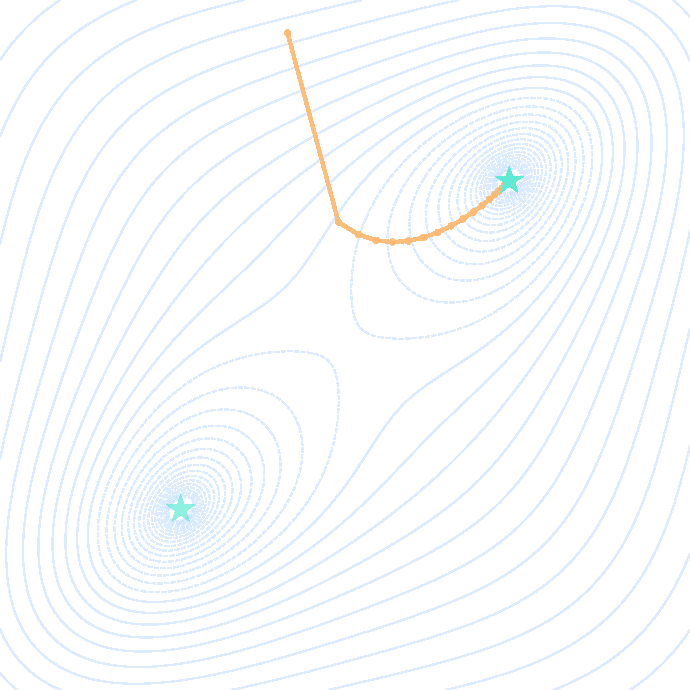
\includegraphics[height=1.05\paperheight]{fig_title_bg}};
    \fill[mNavy, path fading=east] (current page.south west) rectangle ([xshift=-3.4cm]current page.north east);
    \node[anchor=north west, text width=0.62\paperwidth, align=left, inner sep=0pt]
      at ([xshift=1.0cm, yshift=-1.55cm]current page.north west) {%
        {\color{mOrangeLt}\scriptsize\bfseries CSE 402 \,\textperiodcentered\, NUMERICAL ANALYSIS \,\textperiodcentered\, TOPIC 3}\\[10pt]
        {\color{white}\fontsize{28}{30}\selectfont\bfseries \inserttitle}\\[8pt]
        {\color{mSky}\normalsize \insertsubtitle}\\[12pt]
        {\color{mOrangeLt}\rule{2.2cm}{2pt}}\\[14pt]
        {\color{white}\large\bfseries Nawriz Ahmed Turjo}\\[3pt]
        {\color{mSky}\small Roll 2105032 \quad\textperiodcentered\quad \insertdate}};
  \end{tikzpicture}}

% =====================================================================
%  Section dividers: big section number, title, and a "you are here"
%  strip over the 12 stops of the roadmap.
% =====================================================================
\newcommand{\gm@stoplabel}[1]{\ifcase#1 \or The problem\or The gradient\or Derivation\or Step size%
  \or Convergence\or Conditioning\or Failure modes\or Adaptive steps\or Acceleration%
  \or SGD and modern\or Applications\or Part B\fi}
\newcommand{\gm@stop}{\ifcase\value{section} 0\or 1\or 2\or 3\or 3\or 4\or 5\or 5\or 6\or 7\or 8\or 9%
  \or 10\or 10\or 99\or 12\else -1\fi}
\newcommand{\gm@secnum}{\ifcase\value{section}\or 01\or 02\or 03\or 04\or 05\or 06\or 07\or 08\or 09%
  \or 10\or 11\or 12\or 13\or 14\or B\else R\fi}
\newcommand{\gm@stopstrip}{%
  \edef\gm@cur{\gm@stop}%
  \ifnum\gm@cur>-1
  \begin{tikzpicture}[x=0.78cm]
    \draw[mNavy!25, line width=1.2pt] (1,0) -- (12,0);
    \foreach \i in {1,...,12}{%
      \ifnum\gm@cur=99
        \ifnum\i<11 \fill[mNavy] (\i,0) circle (2.6pt);
        \else \fill[mPaper] (\i,0) circle (2.6pt); \draw[mNavy!45, line width=0.8pt] (\i,0) circle (2.6pt); \fi
      \else
        \ifnum\i<\gm@cur \fill[mNavy] (\i,0) circle (2.6pt);
        \else\ifnum\i=\gm@cur
          \fill[mOrange] (\i,0) circle (4.6pt); \fill[mPaper] (\i,0) circle (1.6pt);
          \node[below=5pt, font=\scriptsize\bfseries, mOrange] at (\i,0) {\gm@stoplabel{\i}};
        \else
          \fill[mPaper] (\i,0) circle (2.6pt); \draw[mNavy!45, line width=0.8pt] (\i,0) circle (2.6pt);
        \fi\fi
      \fi}
    \ifnum\gm@cur=99 \node[below=5pt, font=\scriptsize\bfseries, mOrange] at (5.5,0) {Part A recap}; \fi
    \node[left=4pt, font=\tiny, mGrey] at (1,0) {start};
    \node[right=4pt, font=\tiny, mGrey] at (12,0) {Part B};
  \end{tikzpicture}%
  \fi}
\setbeamertemplate{section page}{%
  \begin{minipage}{0.86\textwidth}
    \raggedright
    {\fontsize{46}{46}\selectfont\bfseries\color{mOrange}\gm@secnum}\\[4pt]
    {\usebeamerfont{section title}\usebeamercolor[fg]{section title}\insertsectionhead}\\[2pt]
    {\color{mOrange}\rule{1.6cm}{2pt}}\\[18pt]
    \gm@stopstrip
  \end{minipage}}
\makeatother

% =====================================================================
%  Boxes: a coloured bar on the left instead of a heavy frame.
% =====================================================================
\tcbset{
  gmbase/.style={enhanced, breakable=false, frame hidden, sharp corners,
                 borderline west={2.6pt}{0pt}{#1},
                 colback=#1!6!mPaper, colbacktitle=#1!6!mPaper, coltitle=#1,
                 titlerule=0pt, toptitle=3pt, bottomtitle=-1pt,
                 left=8pt, right=6pt, top=3pt, bottom=4pt,
                 fonttitle=\bfseries\small, fontupper=\small,
                 before skip=5pt, after skip=5pt}
}
\newtcolorbox{probbox}[1][]{gmbase=mOrange, title={#1}}
\newtcolorbox{thmbox}[1][]{gmbase=mNavy, title={#1}}
\newtcolorbox{keybox}[1][]{gmbase=mTeal, title={#1}}
\newtcolorbox{warnbox}[1][]{gmbase=mRed, title={#1}}

% boxed answers: rounded teal outline, same treatment everywhere
\newtcbox{\anstcb}{on line, enhanced, colback=mTeal!8!mPaper, colframe=mTeal, boxrule=0.7pt,
  arc=2.5pt, left=2.5pt, right=2.5pt, top=1pt, bottom=1pt, boxsep=0.6pt}
\newcommand{\ans}[1]{\text{\anstcb{$\displaystyle #1$}}}

% =====================================================================
%  Part B: navy strip with the problem id on the left edge, and step dots
%  in the solution titles.
% =====================================================================
\gdef\gmprob{}
\newcommand{\setprob}[1]{\gdef\gmprob{#1}}
\setbeamertemplate{background}{%
  \ifx\gmprob\empty\else
  \begin{tikzpicture}
    \useasboundingbox (0,0) rectangle (\paperwidth,\paperheight);
    \fill[mNavy] (0,0.8cm) rectangle (0.36cm,\paperheight);   % stops above the footer
    \node[rotate=90, text=white, font=\scriptsize\bfseries, inner sep=0pt] at (0.18cm,0.55\paperheight)
      {PROBLEM \gmprob};
  \end{tikzpicture}%
  \fi}
\makeatletter
\def\gm@dots#1#2#3{%
  \ifnum#1>#3\relax\else
    \ifnum#1>#2\relax{\color{mNavy!25}\textbullet}\else{\color{mOrange}\textbullet}\fi
    \expandafter\gm@dots\expandafter{\the\numexpr#1+1\relax}{#2}{#3}%
  \fi}
\newcommand{\stepdots}[2]{{\normalsize\gm@dots{1}{#1}{#2}}}
\makeatother

% \probtitle{M1}{Stationary points}   -> "Problem M1 · Stationary points"
\newcommand{\probtitle}[2]{Problem #1 \textperiodcentered\ #2}
\newcommand{\soltitle}[3]{Problem #1 \textperiodcentered\ Solution #2/#3 \;\stepdots{#2}{#3}}

% =====================================================================
%  Maths macros
% =====================================================================
\newcommand{\R}{\mathbb{R}}
\newcommand{\E}{\mathbb{E}}
\newcommand{\x}{\mathbf{x}}
\newcommand{\y}{\mathbf{y}}
\newcommand{\e}{\mathbf{e}}
\newcommand{\g}{\mathbf{g}}
\newcommand{\vb}{\mathbf{b}}
\newcommand{\vd}{\mathbf{d}}
\newcommand{\vu}{\mathbf{u}}
\renewcommand{\vv}{\mathbf{v}}   % newtxsf defines a vector accent with this name
\newcommand{\vf}{\mathbf{f}}
\newcommand{\bA}{\mathbf{A}}
\newcommand{\bH}{\mathbf{H}}
\newcommand{\bI}{\mathbf{I}}
\newcommand{\bK}{\mathbf{K}}
\newcommand{\bP}{\mathbf{P}}
\newcommand{\T}{^{\mathsf T}}
\newcommand{\grad}{\nabla f}
\newcommand{\norm}[1]{\left\lVert #1 \right\rVert}
\newcommand{\abs}[1]{\left\lvert #1 \right\rvert}
\newcommand{\ip}[2]{\left\langle #1, #2 \right\rangle}
\newcommand{\lmin}{\lambda_{\min}}
\newcommand{\lmax}{\lambda_{\max}}
\DeclareMathOperator*{\argmin}{arg\,min}
\DeclareMathOperator*{\argmax}{arg\,max}
\DeclareMathOperator{\diag}{diag}

% =====================================================================
%  Statement slides (big idea, dark navy, large type)
% =====================================================================
% \statement{KICKER}{Big sentence}{small follow-up}
\newcommand{\statement}[3]{%
  \begin{frame}[standout]
    \begin{minipage}{0.84\textwidth}\centering
      {\color{mOrangeLt}\scriptsize\bfseries #1\par}\vspace{10pt}
      {\LARGE\bfseries\color{white} #2\par}\vspace{12pt}
      {\color{mOrangeLt}\rule{1.6cm}{1.6pt}\par}\vspace{10pt}
      {\color{mSky}\normalsize\mdseries #3\par}
    \end{minipage}
  \end{frame}}

% =====================================================================
%  Listings style
% =====================================================================
\lstdefinestyle{py}{
  language=Python, basicstyle=\ttfamily\scriptsize,
  keywordstyle=\color{mBlue}\bfseries, commentstyle=\color{mGrey}\itshape,
  stringstyle=\color{mTeal}, showstringspaces=false,
  frame=leftline, framerule=2.6pt, rulecolor=\color{mNavy}, backgroundcolor=\color{mLight},
  xleftmargin=6pt, xrightmargin=2pt, framesep=5pt, columns=fullflexible, keepspaces=true}

% tighter lists and display maths (Fira Sans is taller than the default font)
\setlength{\leftmargini}{1.2em}
\usepackage{etoolbox}
\makeatletter
\newcommand{\gm@tightdisplay}{%
  \setlength{\abovedisplayskip}{5pt plus 2pt minus 2pt}%
  \setlength{\belowdisplayskip}{5pt plus 2pt minus 2pt}%
  \setlength{\abovedisplayshortskip}{2pt plus 2pt}%
  \setlength{\belowdisplayshortskip}{4pt plus 2pt minus 2pt}}
\appto\normalsize{\gm@tightdisplay}
\appto\small{\gm@tightdisplay}
\appto\footnotesize{\gm@tightdisplay}
\makeatother
\setbeamertemplate{itemize/enumerate body begin}{\setlength{\itemsep}{1pt}}
\setbeamertemplate{itemize/enumerate subbody begin}{\setlength{\itemsep}{0pt}}

% numbered bibliography labels (match the [n] citations) instead of icons
\setbeamertemplate{bibliography item}{\insertbiblabel}
% run each entry on as one paragraph (beamer's defaults insert \par between blocks)
\setbeamertemplate{bibliography entry title}{}
\setbeamertemplate{bibliography entry location}{}
\setbeamertemplate{bibliography entry note}{}
